\subsubsection{Q10.14 data 10312021 11092021 grouped by scenario \& PGM}

\begin{comment}
                             EFPR        EO      EFNR     n    pvalue
(frauth, Advantaged)     0.390625  0.609375  0.421875  32.0  0.176937
(frauth, Disadvantaged)  0.350000  0.650000  0.600000  10.0  0.294507
(icu, Advantaged)        0.605263  0.394737  0.605263  19.0  0.059454
(icu, Disadvantaged)     0.352941  0.647059  0.529412  17.0  0.186433
(rent, Advantaged)       0.312500  0.687500  0.437500  16.0  0.051346
(rent, Disadvantaged)    0.456522  0.543478  0.413043  23.0  0.962001
\end{comment}

\begin{table}[h]
    \centering
    \begin{tabular}{|c|c|c|c|c|c|c|}
        \hline
        scenario & PGM & EFPR & EO & EFNR & n & p-value\\
        \hline
        frauth & Advantaged & 0.391 & \textbf{0.609} & 0.422 & 32.0 & 0.177\\
		frauth & Disadvantaged & 0.350 & \textbf{0.650} & \textbf{0.600} & 10.0 & 0.295\\
		icu & Advantaged & \textbf{0.605} & 0.395 & \textbf{0.605} & 19.0 & 0.059\\
		icu & Disadvantaged & 0.353 & \textbf{0.647} & \textbf{0.529} & 17.0 & 0.186\\
		rent & Advantaged & 0.312 & \textbf{0.688} & 0.438 & 16.0 & 0.051\\
		rent & Disadvantaged & 0.457 & \textbf{0.543} & 0.413 & 23.0 & 0.962\\
		
        \hline
    \end{tabular}
    \caption{Grouped by scenario PGM}
    \label{tab:my_label}
\end{table}
\begin{figure}[h]
    \centering
    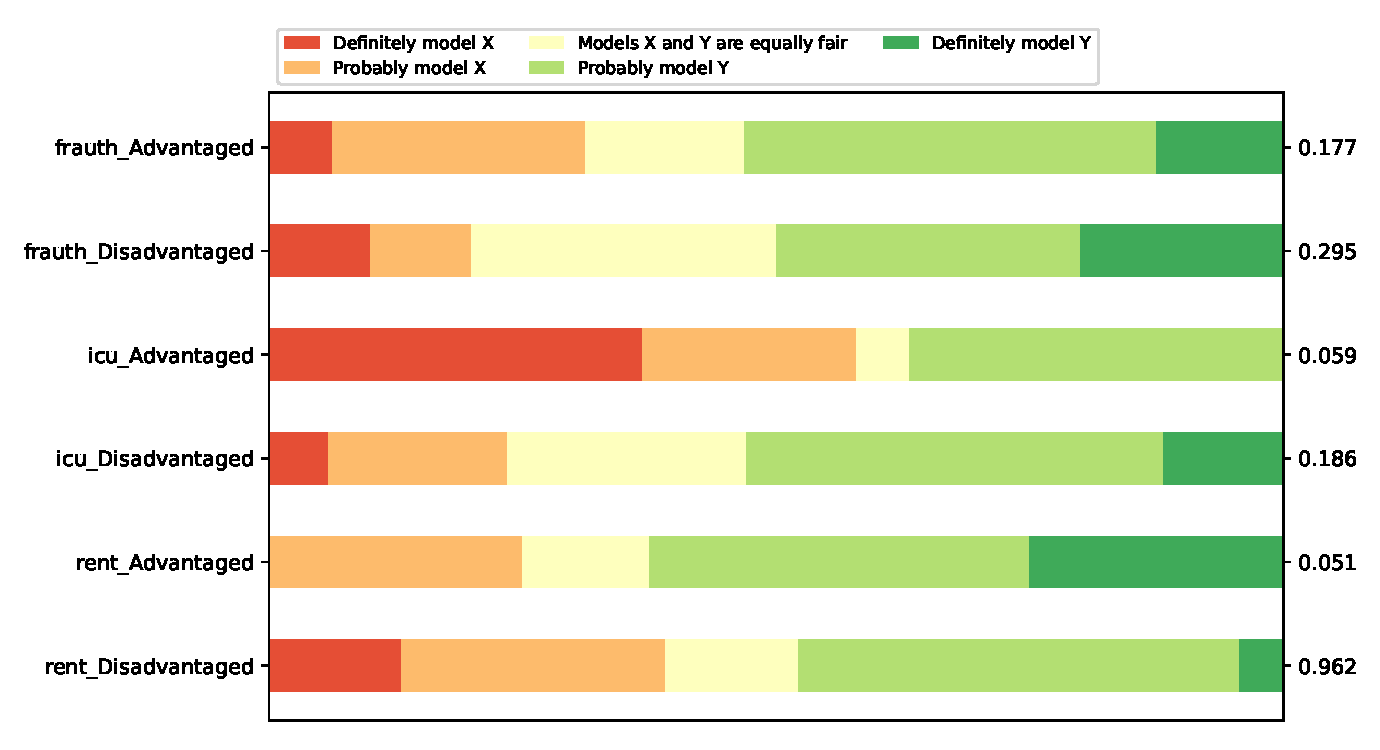
\includegraphics[width=0.8\textwidth]{figures/Q10.14/10312021_11092021/Q10.14_scenario_PGM.pdf}
    \caption{Grouped by scenario \& PGM}
    \label{fig:my_label}
\end{figure}
